%========================================================
\chapter{High Level Design}
%========================================================

This Chapter presents the high level design of the proposed TBML detection framework including architectural approaches, design aspects related to the software and the
entire system architecture combining the capabilities of graph-based fraud detection, federated learning, and real-time transaction monitoring in the unified compliance solution.

%========================================================
\section[Design Considerations]{\textbf{Design Considerations}}
%========================================================

A number of operational, analytical and security-related factors affect the design of the
proposed TBML detection framework due to the nature of Trade-Based Money
Laundering which includes complex interconnections between different financial
organizations and their transactions. Therefore, the architecture of the proposed
solution has to address the requirements for large-scale analytical processing and
secure collaboration between the institutions, as well as the ability to efficiently perform
graph-based fraud analysis. The key design considerations of the proposed
framework are discussed in the following subsections.

%========================================================
\subsection[General Considerations]{\textbf{General Considerations}}
%========================================================
The proposed TBML detection framework is designed to analyze large transaction volumes from multiple financial organizations. Since laundering schemes always include
interconnected accounts, trade companies, invoices, and other relationships, the framework employs graph-based modeling approaches that allow for better representation of the hidden financial dependencies compared to traditional relational models.
Additionally, the architecture of the proposed framework allows for real-time
transaction processing.

Security, privacy protection, and the scalability of the system have to be considered as critical aspects of the proposed architecture since financial and compliance-related data will need to be handled. In order to fulfill the stated requirements, the framework will include secure authentication techniques, role-based access controls, and federated learning approaches for protected cooperation across organizations without exposing transactional information. System design is based on the use of modular architecture to facilitate easier implementation, maintenance, and future enhancements to transaction monitoring, fraud detection, compliance reporting, and dashboards visualization services

%========================================================
\subsection[Development Methods]{\textbf{Development Methods}}
%========================================================
The proposed TBML detection framework is designed in a modular and iterative style of development to enable scalable system integration for future continuous development and improvement of analytical functionalities. Individual system components, such as transaction monitoring services, graph construction pipelines, fraud detection models, federated learning environments, and dashboard interfaces are built and tested separately from the rest of the system and then incorporated into the full monitoring system.

The development process also involves iterative modelling evaluation and experimentation, which will enhance fraud detection performance and analytical reliability. Processed transactional data are used for training graph-based machine learning models, while the use of API-based communication mechanisms enables the integration of frontend and backend services to enable real-time interaction between the monitoring modules and the analytical services.

From the beginning of implementation, version control and collaborative development practices are used to manage the backend services, machine learning workflows, front-end interfaces, and analytical configurations in an efficient way. This is the modular development approach, which will facilitate the debugging, testing, maintenance and further development of the proposed framework for fraud detection.
%========================================================
\section[Architectural Strategies]{\textbf{Architectural Strategies}}
%========================================================

The architectural approaches taken in the proposed TBML detection framework aim at providing scalable financial transaction analysis, secure collaboration between institutions, and efficient communication between analytical services and monitoring interfaces. All these components, including graph-based models, backend analytical services, real-time dashboards, and distributed learning mechanisms are combined into a single monitoring environment. Some major architectural schemes related to the proposed framework are discussed in the following subsections.

%========================================================
\subsection[Programming Language]{\textbf{Programming Language}}
%========================================================

The proposed TBML detection framework primarily utilizes Python for backend services, graph processing, machine learning workflows, and analytical computations. Python was selected due to its extensive support for deep learning libraries, graph analytical frameworks, and federated learning environments. Libraries such as PyTorch, PyTorch Geometric, and Flower are utilized for implementing graph neural network models and distributed learning mechanisms within the fraud detection framework.

The frontend monitoring dashboard is built with Next.js and React.js for responsive UI development and real-time analytical visualization. Implementing dashboard components, transaction monitoring interfaces and compliance management services are done in JavaScript and TypeScript. FastAPI is also built-in to enable communication between front-end dashboards, back-end services, and machine learning modules via APIs.

%========================================================
\subsection[System Integration Architecture]{\textbf{System Integration Architecture}}
%========================================================
The proposed TBML detection framework is mainly based on Python as a back-end, graph processing, machine learning pipeline and analytical computation language. The decision to use Python was made because of its support with deep learning libraries, graph analytical frameworks, and federated learning environments. In this framework, the fraud detection models and distributed learning mechanisms are implemented using libraries like PyTorch, PyTorch Geometric, and Flower, which are used for implementing graph neural network models and distributed learning mechanisms within the framework of fraud detection

%========================================================
\subsection[Data Storage Management]{\textbf{Data Storage Management}}
%========================================================

The proposed TBML detection framework utilizes both relational and graph-based database systems to support efficient financial data management and analytical processing. PostgreSQL is utilized for storing structured transactional records, authentication information, compliance-related data, and generated Suspicious Transaction Reports. The relational database environment supports secure storage and efficient retrieval of operational monitoring information within the framework.

Memgraph is utilized as the graph database environment for storing interconnected financial entities and transactional relationships. Accounts, organizations, invoices, and transactions are represented as graph nodes and edges to support relational fraud analysis and graph neural network processing. The combined relational and graph-based storage strategy improves scalability, analytical flexibility, and efficient synchronization between backend analytical services and monitoring dashboards.

%========================================================
\section[Overall System Architecture]{\textbf{Overall System Architecture}}
%========================================================
The proposed TBML detection framework is aimed at providing intelligence to enable
intelligent financial transaction monitoring, relational fraud analysis, federated learning, and compliance reporting on TBML cases. The system encompasses transaction processing,
construction of a heterogeneous graph, fraud detection through machine learning algorithms, and monitoring of suspicious TBML transactions.
The architecture starts from multiple data sources like bank systems,
trade systems, and external financial service providers. The transaction data, trade information,
KYC details, and monitoring activities are then captured and passed through a transaction
processing module responsible for performing data validation, cleaning, normalization,
and event creation. The cleaned data is then transformed into heterogeneous graph structures where the entities like accounts, organizations, invoices, and transactions are modeled in terms of interconnected nodes and edges. It helps in identifying the hidden financial relations and suspicious transactions needed for learning from graphs.
The fraud detection framework includes Hybrid Graph Neural Network for relation analysis and temporal learning for transactional analysis. Both of these techniques are helpful in capturing complex launderers' behavior and improving the accuracy of fraud detection based on risk predictions. For ensuring the privacy of the data, federated learning is employed in this architecture, where all institutions train their models locally but share only their model parameters with the global aggregation module.

The aggregated global model is used in the inference and risk scoring module to classify the transactions as suspicious transactions and produce the risk scores of fraud. High-risk transactions would be sent to the compliance management module in order to trigger alerts, Suspicious Transaction Report generation, and regulations support. The total architecture of the proposed TBML detection framework is shown in Figure 4.1.Figure 4.1: Overall Architecture of the Proposed TBML Detection Framework 4.4 Data Flow Diagrams

\begin{figure}[H]
    \centering
    \fbox{
        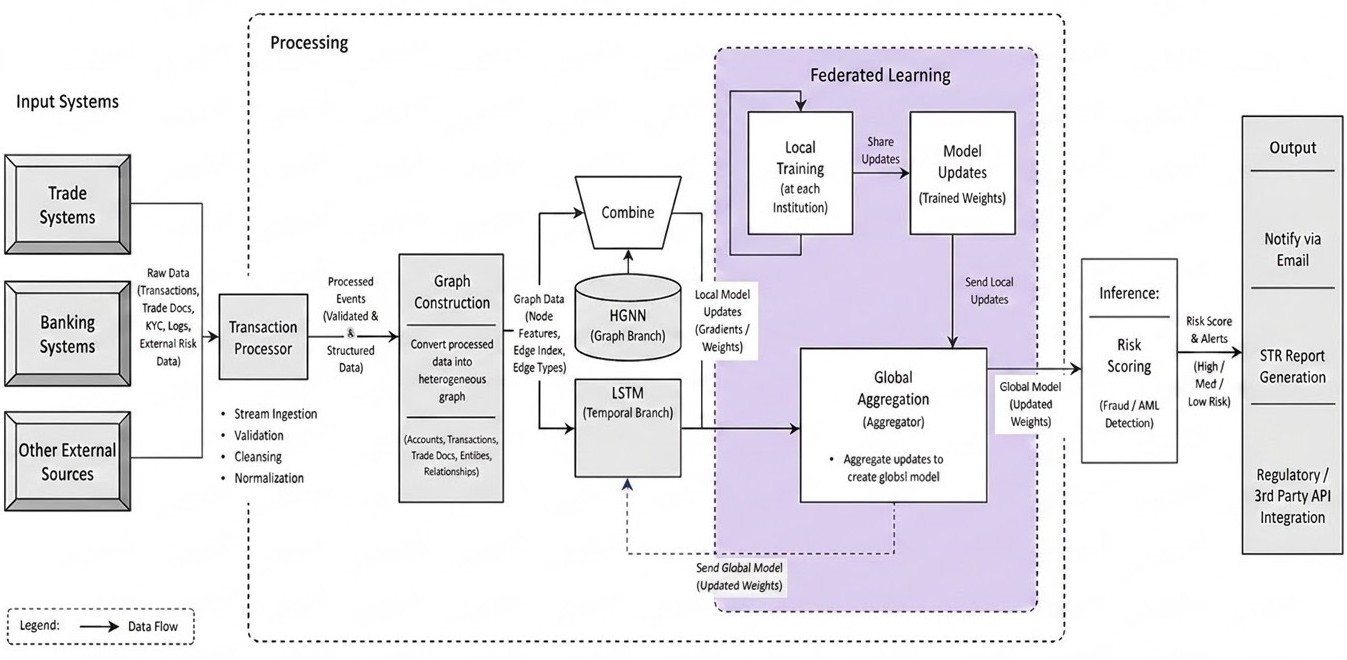
\includegraphics[width=0.98\textwidth]{Figures/overall_architecture.jpg}
    }
    \caption{Overall Architecture of the Proposed TBML Detection Framework}
    \label{fig:overall_architecture}
\end{figure}

%========================================================
\section[Data Flow Diagrams]{\textbf{Data Flow Diagrams}}
%========================================================

Data Flow Diagram (DFD) is the graphical tool used to present the movement of
data within a system and interactions among process, external entity, and data store.
DFDs are useful in illustrating the flow of information through system architecture in terms of data entry, data processing, data storage, and data transfer. Within the proposed Federated Heterogeneous Graph Neural Network (HGNN)-Based Trade-Based Money Laundering (TBML) Detection System, DFDs have been used to describe the entire workflow including transaction gathering, graph building, federated learning, fraud analysis, and alert generation. Decomposing the system architecture into Level 0, Level 1, and Level 2 diagrams helps gain a deeper insight about operation flow, subsystem interaction, and data processing.

%========================================================
\subsection[Data Flow Diagram Level 0]{\textbf{Data Flow Diagram Level 0}}
%========================================================

\begin{figure}[H]
    \centering
    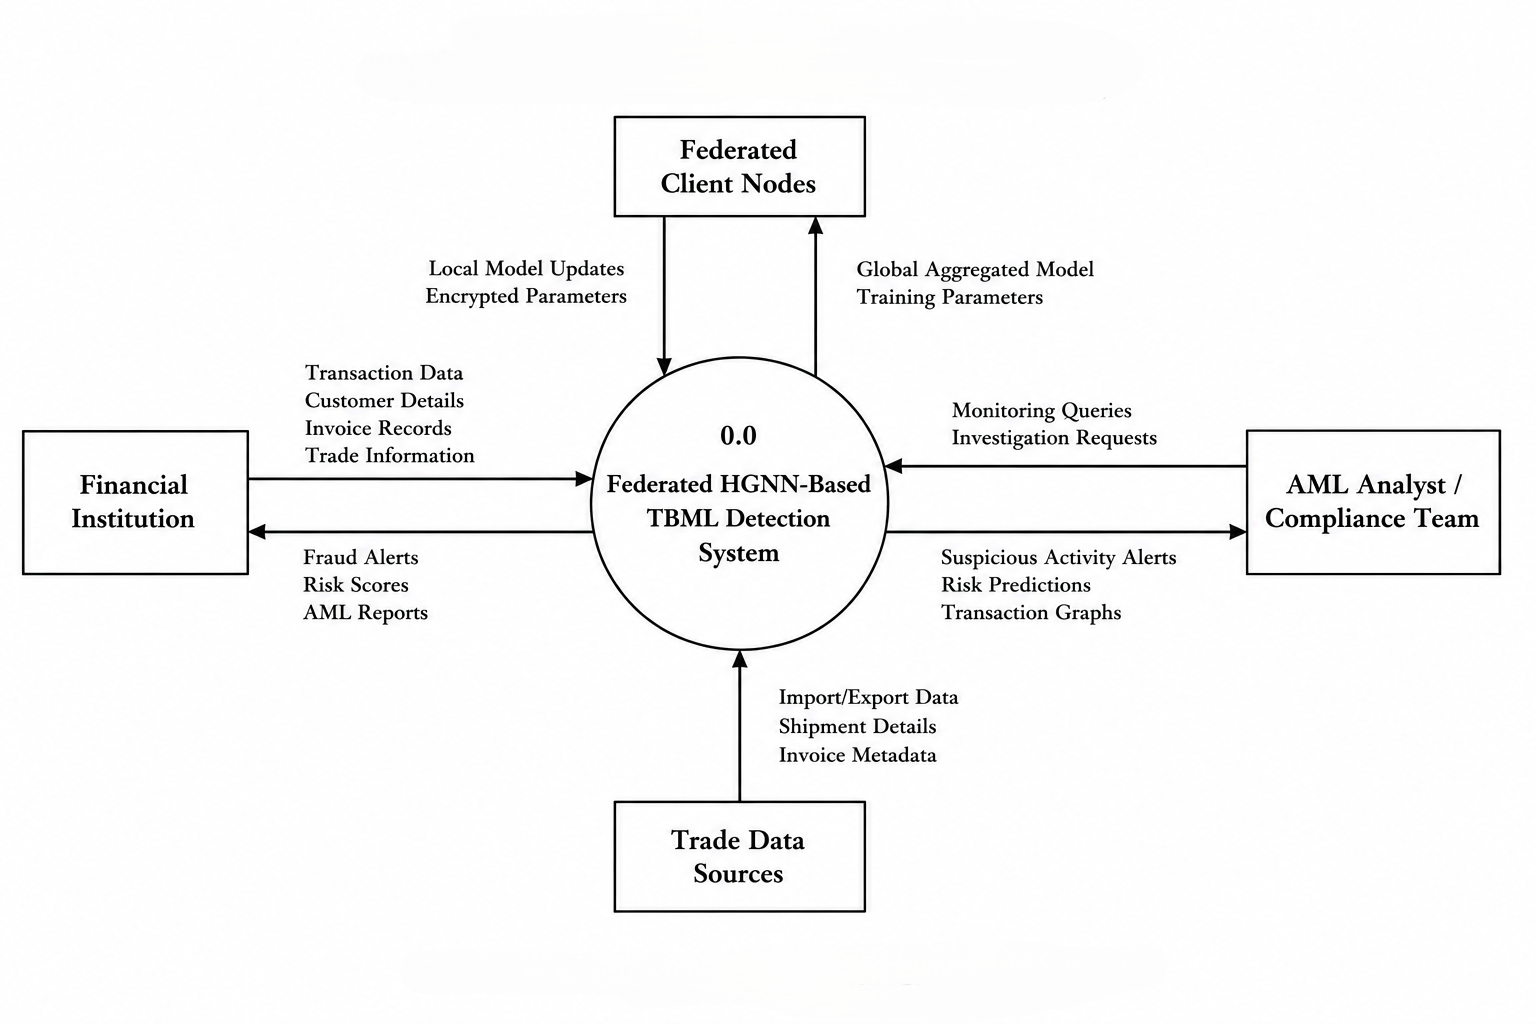
\includegraphics[width=0.95\linewidth]{Figures/DFD_Level_0.png}
    \caption{Level 0 Data Flow Diagram}
    \label{fig:dfd_level0}
\end{figure}

Figure \ref{fig:dfd_level0} shows the Level 0 Data Flow Diagram of the suggested Federated HGNN-Based TBML Detection System. This diagram serves as a high-level context-based representation of the entire system operating as one process involving various external participants such as Financial Institutions, Federated Client Nodes, AML Analysts, and Trade Data Sources. Financial Institutions supply transactions data, customers' data, invoice data, and other relevant data for processing by the system. Trade Data Sources offer the necessary import-export data and shipping information needed for transaction validation and graph creation. Federated Client Nodes share their locally trained model weights, which are then aggregated for global model training. Using these inputs, the system creates alerts, risks predictions, AML reports, and suspicious activities notifications that could be useful for compliance officers and financial analysts.
%========================================================
\subsection[Data Flow Diagram Level 1]{\textbf{Data Flow Diagram Level 1}}
%========================================================

\begin{figure}[H]
    \centering
    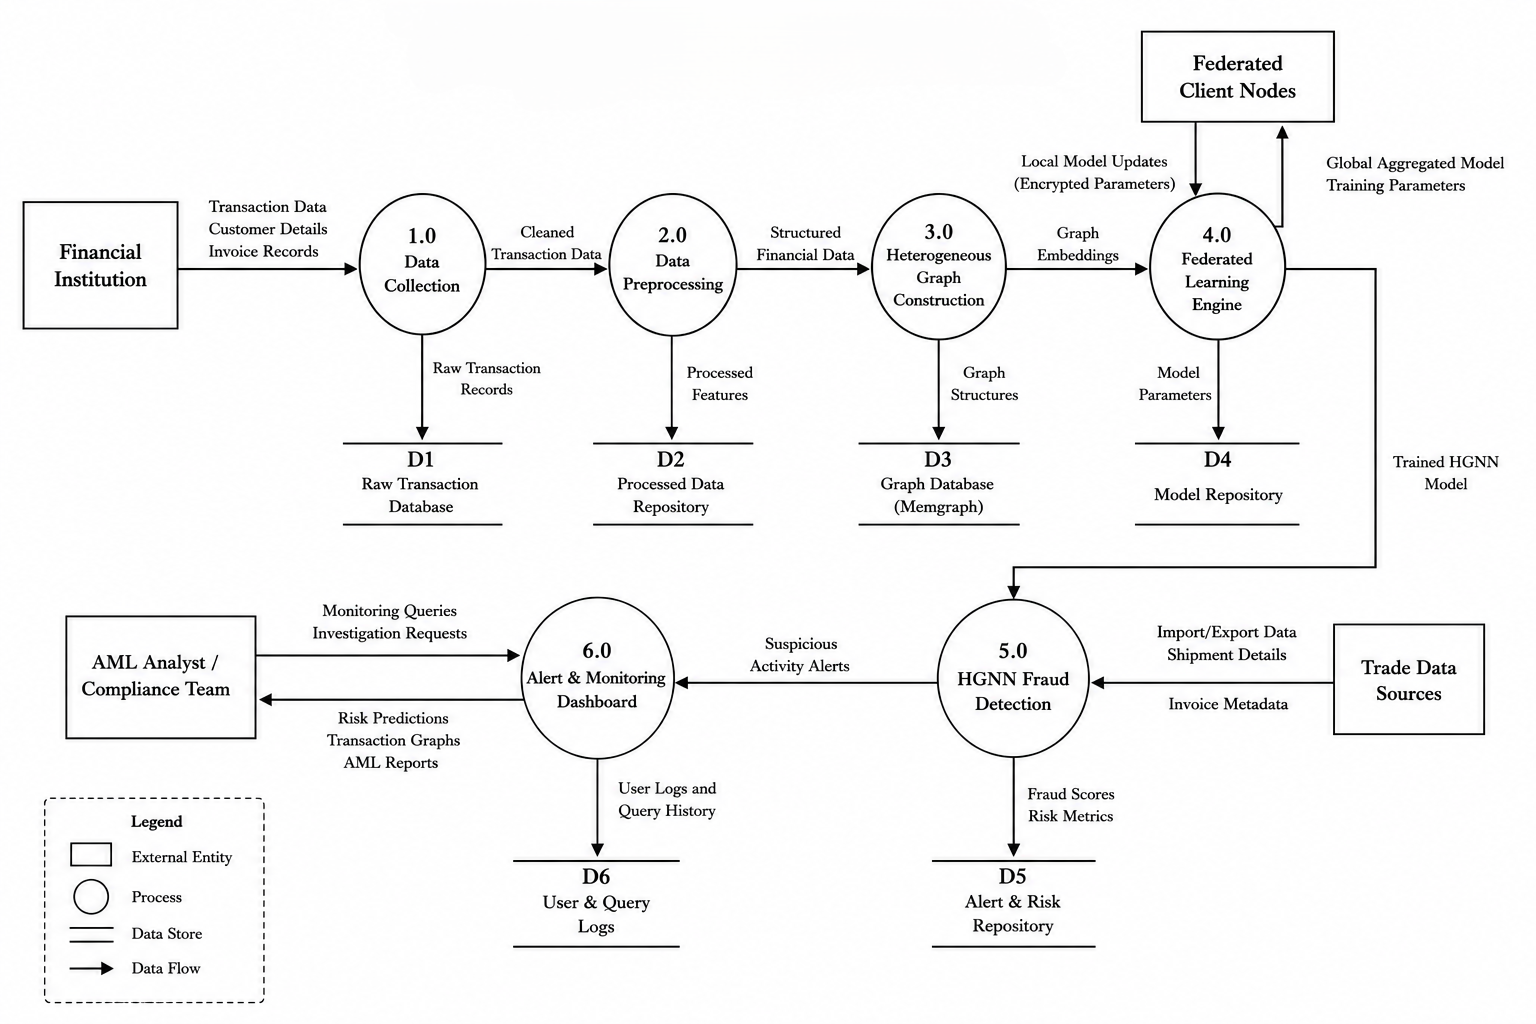
\includegraphics[width=\linewidth]{Figures/DFD_Level_1.png}
    \caption{Level 1 Data Flow Diagram}
    \label{fig:dfd_level1}
\end{figure}

Figure \ref{fig:dfd_level1} illustrates the level 1 data flow diagram of the designed TBML detection framework is illustrated through breaking down the main system architecture into several
processes. In particular, the architecture is made up of different modules including
Data Collection, Data Preprocessing, Heterogeneous Graph Construction,
Federated Learning Engine, HGNN Fraud Detection, and Alert and Monitoring
Dashboard. The Data Collection module is responsible for fetching raw transactional data and customer data from financial institutions; such data are cleaned and preprocessed to create structured financial features that can be used for building a heterogeneous
graph representation by graph construction engines in the graph database. As such,
the federated learning engine engages in conducting distributed collaborative model
training by using the encrypted local updates sent by federated clients without
violating the data privacy of institutions. The generated HGNN models are then used
by the fraud detection engine to detect any suspicious transaction, compute the fraud
scores, and raise alerts. Lastly, the investigation can be carried out by AML analysts
and compliance teams through the dashboard system.


%========================================================
\subsection[Data Flow Diagram Level 2]{\textbf{Data Flow Diagram Level 2}}
%========================================================
\begin{figure}[H]
    \centering
    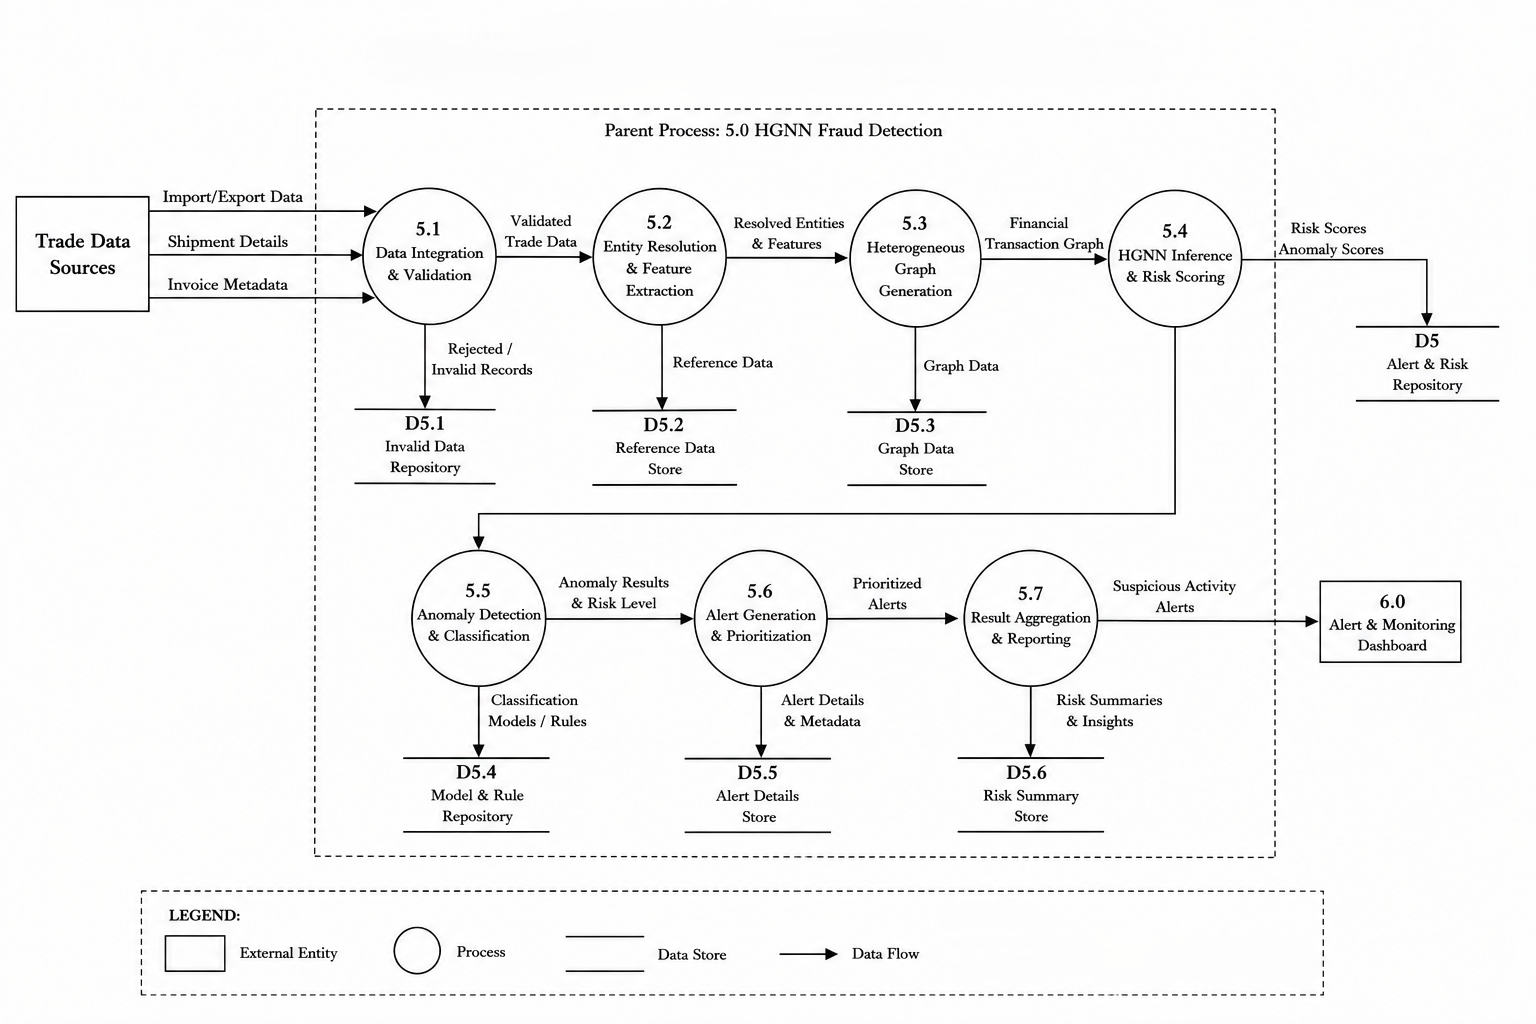
\includegraphics[
        width=\textwidth,
        height=0.9\textheight,
        keepaspectratio
    ]{Figures/DFD_Level_2.png}
    \caption{Level 2 Data Flow Diagram}
    \label{fig:dfd_level2}
\end{figure}

Figure \ref{fig:dfd_level2}
depicts the Level 2 Data Flow Diagram showing the internal decomposition of the HGNN Fraud Detection module in the proposed framework.
The
initial stage of the process involves Data Integration and Validation, during which data from various sources related to trade invoices, shipments, and transaction
metadata is integrated and validated for discrepancies. The
valid data is fed into the Entity Resolution and Feature Extraction stage, where relational attributes are identified, and financial contextual features are extracted
for the purposes of graph-based learning. The next process stage involves Heterogeneous Graph Generation, where interconnected financial transaction graphs
are created, containing the relevant information about entities, accounts, invoices, and trade relations. The HGNN Inference and Risk Scoring module utilizes
graph-based neural network learning to determine anomaly scores and detect any suspicious transaction patterns. The results of this analysis are processed
by the Anomaly Detection and Classification module, followed by the Alert Generation and Prioritization module, where suspicious activities are prioritized based on
risk levels. Finally, the Result Aggregation and Reporting module prepares a report of the detected fraudulent activities, suspicious transaction patterns, and
analytical results and forwards it to the Alert and Monitoring Dashboard module.


%========================================================
\section{Summary}
%========================================================
In this chapter, the high-level architecture of the proposed Federated Heterogeneous Graph Neural Network (HGNN)-Based TBML Detection Framework is described. Design issues involved scaling, privacy preservation, modularity, transaction monitoring, and secure collaboration among institutions in a distributed environment. Besides the discussion of design issues, the chapter explained how the design methodologies, architectural approaches, programming tools, and integration techniques used for the implementation of graph-based fraud detection, federated learning, and compliance monitoring were developed.
System Architecture
The complete system architecture revealed the integration of the processing of transactions, heterogeneity graph generation, hybrid graph neural networks, federated learning approach, and compliance environment for effective TBML detection. In addition, the level 0, level 1, and level 2 Data Flow Diagrams depicting the flow of financial transactions, internal processing, fraud detection, and alerts are provided in the chapter. All the architectural components combine together to provide a scalable and privacy-preserving monitoring system for anti-money laundering.
